%%%%%%%%%%%%%%%%%%%%%%%%%%%%%%%%%%%%%%%%%
% Beamer Presentation
% LaTeX Template
% Version 1.0 (10/11/12)
%
% This template has been downloaded from:
% http://www.LaTeXTemplates.com
%
% License:
% CC BY-NC-SA 3.0 (http://creativecommons.org/licenses/by-nc-sa/3.0/)
%
%%%%%%%%%%%%%%%%%%%%%%%%%%%%%%%%%%%%%%%%%

%----------------------------------------------------------------------------------------
%	PACKAGES AND THEMES
%----------------------------------------------------------------------------------------

\documentclass{beamer}
\usepackage[utf8]{inputenc}

\usepackage{media9}

\mode<presentation> {

% The Beamer class comes with a number of default slide themes
% which change the colors and layouts of slides. Below this is a list
% of all the themes, uncomment each in turn to see what they look like.

%\usetheme{default}
%\usetheme{AnnArbor}
%\usetheme{Antibes}
%\usetheme{Bergen}
%\usetheme{Berkeley}
%\usetheme{Berlin}
\usetheme{Boadilla}
%\usetheme{CambridgeUS}
%\usetheme{Copenhagen}
%\usetheme{Darmstadt}
%\usetheme{Dresden}
%\usetheme{Frankfurt}
%\usetheme{Goettingen}
%\usetheme{Hannover}
%\usetheme{Ilmenau}
%\usetheme{JuanLesPins}
%\usetheme{Luebeck}
%\usetheme{Madrid}
%\usetheme{Malmoe}
%\usetheme{Marburg}
%\usetheme{Montpellier}
%\usetheme{PaloAlto}
%\usetheme{Pittsburgh}
%\usetheme{Rochester}
%\usetheme{Singapore}
%\usetheme{Szeged}
%\usetheme{Warsaw}

% As well as themes, the Beamer class has a number of color themes
% for any slide theme. Uncomment each of these in turn to see how it
% changes the colors of your current slide theme.

%\usecolortheme{albatross}
%\usecolortheme{beaver}
%\usecolortheme{beetle}
%\usecolortheme{crane}
%\usecolortheme{dolphin}
%\usecolortheme{dove}
%\usecolortheme{fly}
%\usecolortheme{lily}
%\usecolortheme{orchid}
\usecolortheme{rose}
%\usecolortheme{seagull}
%\usecolortheme{seahorse}
%\usecolortheme{whale}
%\usecolortheme{wolverine}

%\setbeamertemplate{footline} % To remove the footer line in all slides uncomment this line
%\setbeamertemplate{footline}[page number] % To replace the footer line in all slides with a simple slide count uncomment this line

%\setbeamertemplate{navigation symbols}{} % To remove the navigation symbols from the bottom of all slides uncomment this line
}

\usepackage{graphicx} % Allows including images
\usepackage{booktabs} % Allows the use of \toprule, \midrule and \bottomrule in tables

%----------------------------------------------------------------------------------------
%	TITLE PAGE
%----------------------------------------------------------------------------------------

\title[Distributed System]{Distributed System} % The short title appears at the bottom of every slide, the full title is only on the title page

\author[Cereda Cella Cimbelli]{Stefano Cereda\\ Leonardo Cella\\ Alessandro Cimbelli} % Your name
\institute[Polimi] % Your institution as it will appear on the bottom of every slide, may be shorthand to save space
{
Politecnico di Milano \\ % Your institution for the title page
\medskip
\textit{} % Your email address
}
\date{\today} % Date, can be changed to a custom date

\begin{document}

\begin{frame}
\titlepage % Print the title page as the first slide
\end{frame}

\begin{frame}
\frametitle{Overview} % Table of contents slide, comment this block out to remove it
\tableofcontents % Throughout your presentation, if you choose to use \section{} and \subsection{} commands, these will automatically be printed on this slide as an overview of your presentation
\end{frame}

%----------------------------------------------------------------------------------------
%	PRESENTATION SLIDES
%----------------------------------------------------------------------------------------

%------------------------------------------------
\section{Introduzione} % Sections can be created in order to organize your presentation into discrete blocks, all sections and subsections are automatically printed in the table of contents as an overview of the talk
%------------------------------------------------

\subsection{Traccia Scelta} % A subsection can be created just before a set of slides with a common theme to further break down your presentation into chunks

\begin{frame}
	\frametitle{Traccia Scelta}
	
	Il progetto che abbiamo deciso di sviluppare è:
	\begin{itemize}
		\item Distributed, topic-based publish/subscribe with causal consistency
	\end{itemize}
	
	Il quale è stato realizzato tramite OmNet++.
	
\end{frame}

\subsection{Assunzioni}

\begin{frame}
	\frametitle{Assunzioni}
	
	Nel realizzare la traccia abbiamo fatto le seguenti assunzioni:
	\begin{itemize}
		\item Quando un broker smette di funzionare si comporta come un hub.
		\item Canali sicuri.
		\item Che la rete simulata sia quella di un overlay network e che sia aciclica per costruzione.
	\end{itemize}
\end{frame}



%------------------------------------------------
\section{Simulazione casistiche}
%------------------------------------------------
\subsection{Client Leave/join}

\begin{frame}
\frametitle{Client Leave/join}

Vediamo adesso i punti salienti della simulazione della client leave/join:
\begin{itemize}
	\item Fase di inizializzazione della rete.
	\item Funzionamento \emph{normale} della rete con scambio di messaggi.
	\item \emph{Client1} performa una leave.
	\item La rete aggiorna le proprie tabelle di routing considerando che il client1 si sia disconnesso.
	\item \emph{Client} pubblica messaggi che sarebbero arrivati al \emph{client1} ma che adesso, giustamente, non gli giungono più.
	\item Il \emph{client1} torna a far parte della rete con una join.
	\item Il \emph{client1} riceve adesso correttamente i messaggi a cui era interessato.
\end{itemize}
\end{frame}

\begin{frame}

	
	\includemedia[activate=pageopen,addresource=Video/clientleavejoin.flv,windowed=1024x768,flashvars={source=Video/clientleavejoin.flv}]{}{VPlayer.swf}

\end{frame}

\subsection{Broker Leave/join}

\begin{frame}
	\frametitle{Broker Leave/join}
	
	Vediamo adesso i punti salienti della simulazione della broker leave/join:
	\begin{itemize}
		\item Fase di inizializzazione della rete.
		\item Funzionamento \emph{normale} della rete con scambio di messaggi correttamente inoltrati secondo le subscriptions.
		\item \emph{Broker} performa una leave ed entra in \emph{hub mode}.
		\item La rete continua a funzionare senza il contributo di \emph{broker}.
		\item \emph{Broker} effettua una join e, i broker vicini, gli comunicano quali sono le subscriptions a cui è interessato.
		\item La rete torna a funzionare come prima della leave, con un corretto inoltro dei messaggi da parte di \emph{broker}.
	\end{itemize}
\end{frame}

\begin{frame}
	
		\includemedia[activate=pageopen,addresource=Video/brokerleavejoinofficial.flv,windowed=1024x768,flashvars={source=Video/brokerleavejoinofficial.flv}]{}{VPlayer.swf}
	
\end{frame}

\subsection{Causal Consistency}
\begin{frame}
	\frametitle{Causal Consistency}
	
		\begin{figure}[h!]
			\centering
			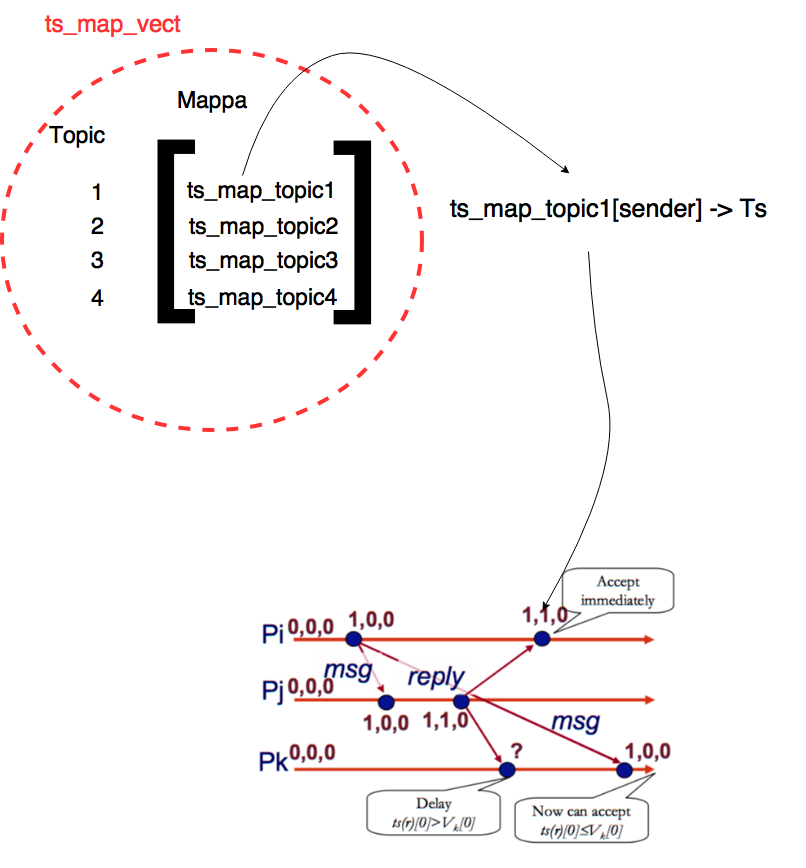
\includegraphics{Risorse/cc.png} %
			\caption{File Causal Consistency structure}
		\end{figure}
		
\end{frame}

\begin{frame}
	\frametitle{Causal Consistency Comparison}
	
	\begin{itemize}
		\item Per la \emph{Causal Consistency} abbiamo utilizzato dei \emph{vector clock} la cui lunghezza varia dinamicamente con il comportamento della rete. Infatti nel nostro modello il numero di client può variare dinamicamente ed non è noto a priori. La regole che governano i vector clock per ottenere la \emph{causal consistency} restano immutate ad eccezione della regola:\\
		
		\begin{center}
			$ts\left ( r \right )\left [ i \right ] \leq V_k$  $ \forall i \neq j$
		\end{center}
		
		
		 La regola generale descritta sopra è estesa nel caso si verifichino i seguenti casi:
		\begin{itemize}
			\item Se il messaggio contiene timestamp di clients non conosciuti dal ricevente, allora esso non sarà \emph{causal consistent}. (Potremmo dover ancora ricevere dei messaggi dai suddetti clienti)
			\item Se il messaggio contiene timestamp di clients conosciuti solo dal ricevente, questo non influenzerà la consistenza.
		\end{itemize}
	\end{itemize}
	
\end{frame}

\section{Statistiche}

\begin{frame}
	\Huge{\centerline{Statistiche}}
\end{frame}

\subsection{Statistiche Broker}
\begin{frame}
	\frametitle{Statistiche Broker}
	
	\begin{figure}[h!]
		\centering
		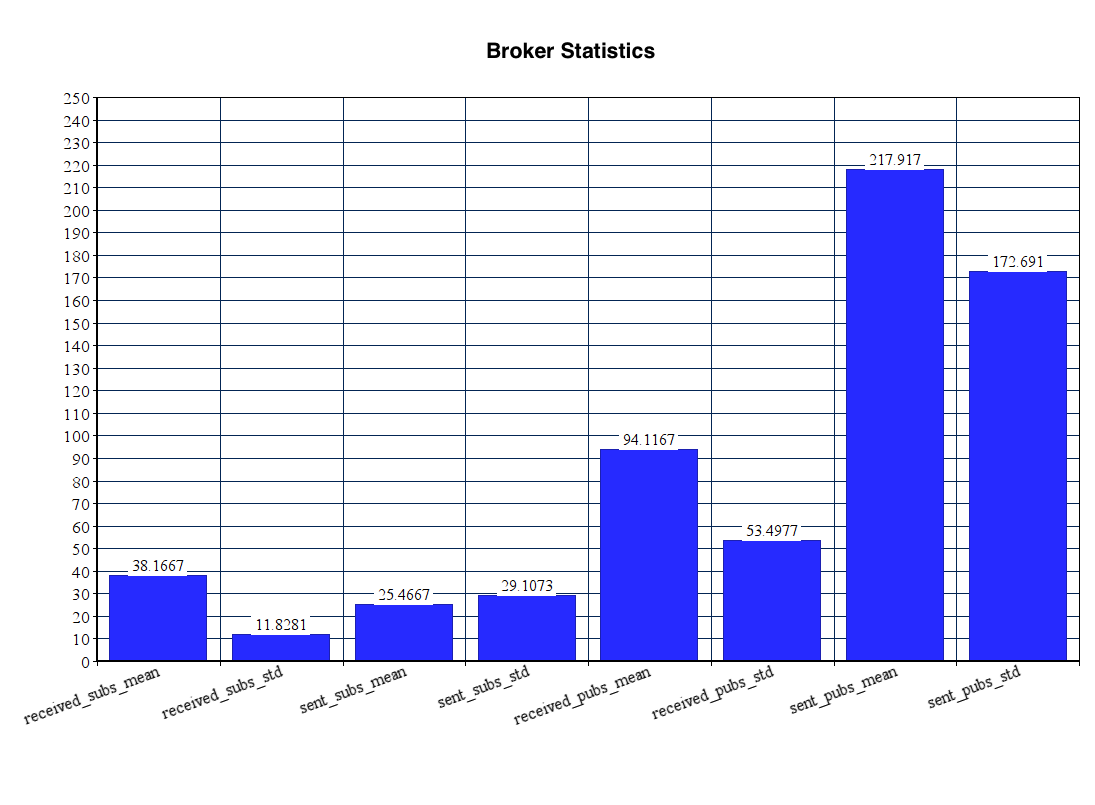
\includegraphics{Risorse/broker_stats.png} %
		\caption{File Broker Statistics}
	\end{figure}
	
\end{frame}

\subsection{Statistiche Client}
\begin{frame}
	\frametitle{Statistiche Client}
	
	\begin{figure}[h!]
		\centering
		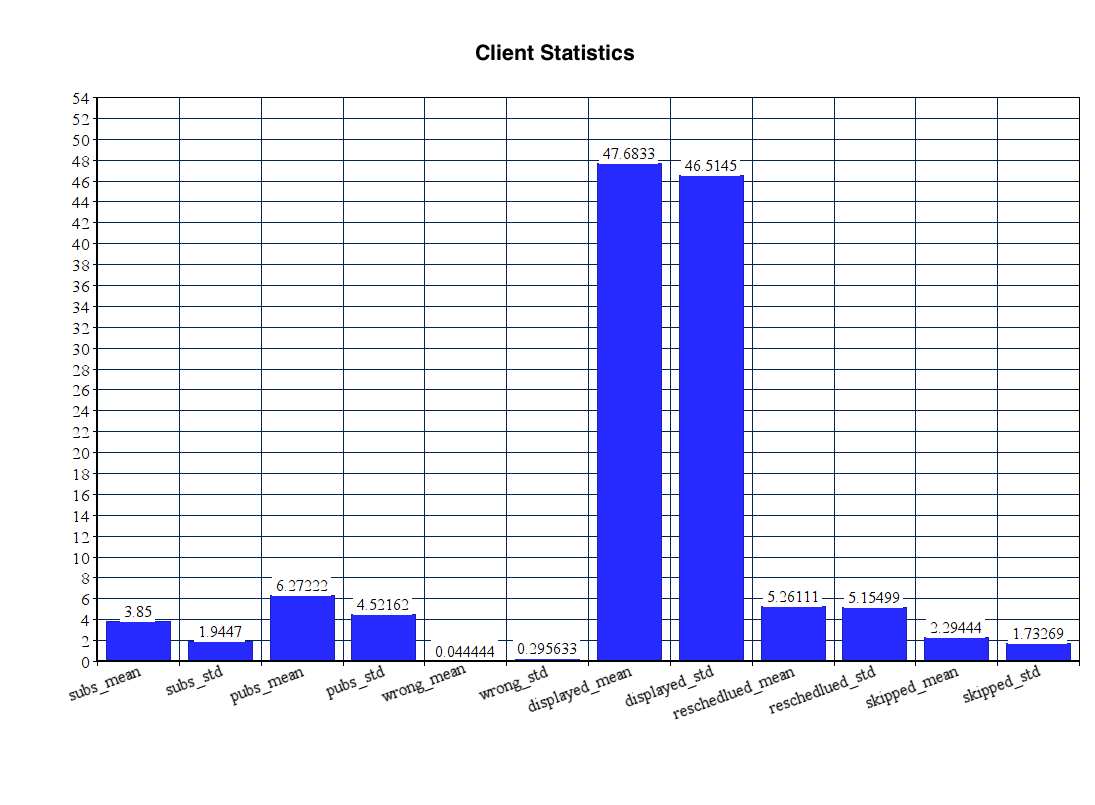
\includegraphics{Risorse/client_stats.png} %
		\caption{File Client Statistics}
	\end{figure}
	
\end{frame}

%Video/client_leave_join.mp4
\section{Conclusione}
\begin{frame}
	\Huge{\centerline{Fine}}
\end{frame}

%----------------------------------------------------------------------------------------

\end{document} 